% =============================================================================
% Kapitel 5: Systementwurf
% =============================================================================

Aufbauend auf der Analyse des bestehenden Systems (Kap.~\ref{sec:vorarbeit}) und den definierten Anforderungen (Kap.~\ref{sec:anforderungen}) wird in diesem Kapitel der Entwurf des erweiterten Systems dargelegt.
Dabei wird zunächst die Gesamtarchitektur beschrieben, anschließend das hybride Cascading-Muster im Detail erläutert und abschließend die wesentlichen Technologieentscheidungen begründet.

\subsection{Gesamtarchitektur}\label{sec:architektur}

Die Architekturentscheidung ergibt sich aus zwei Randbedingungen: Erstens erfordert das gewählte Sentence-Embedding-Modell mit 278 Millionen Parametern eine serverseitige Inferenz -- eine Ausführung im Browser ist aufgrund der Modellgröße und des Speicherbedarfs nicht praktikabel.
Zweitens sollen die trainierten SVM-Klassifikatoren und die Referenzdatenbank zentral vorgehalten werden, um konsistente Analyseergebnisse zu gewährleisten.
Daraus resultiert eine Zwei-Komponenten-Architektur aus einem Browser-Frontend und einem Python-Backend, die über eine REST-API kommunizieren.

Abb.~\ref{fig:architektur-gesamt} zeigt die Gesamtarchitektur.
Das \textbf{Frontend} ist eine Single-Page-Application auf Basis von Nuxt~4 und Vue~3.
Es besteht aus drei Hauptbereichen: dem Tiptap-Editor mit Echtzeit-Verb-Highlighting, einem Analyse-Panel, das pro Satz Typ, Taxonomiestufe, Konfidenz und Quelle anzeigt, sowie einer Set-Analyse-Übersicht, die die Taxonomie-Verteilung auf Modulebene darstellt.
Bei jeder Texteingabe sendet das Frontend nach einer Debounce-Pause den vollständigen Text über die REST-API an das Backend.

Das \textbf{Backend} ist ein Python-Service auf Basis von FastAPI.
Es stellt einen einzigen Analyse-Endpunkt bereit (\texttt{POST /api/analyze}), der den Eingabetext entgegennimmt und ein strukturiertes Ergebnis zurückgibt.
Intern orchestriert eine Hybrid-Analyse-Pipeline sechs Verarbeitungsschritte (vgl. Kap.~\ref{sec:cascading-entwurf}).
Beim Start des Services werden alle benötigten Modelle und Daten in den Speicher geladen: das SBERT-Modell für die Embedding-Berechnung, die beiden SVM-Klassifikatoren für Typ- und Taxonomie-Zuordnung, die vorberechneten Referenz-Embeddings sowie das spaCy-Modell für linguistische Vorverarbeitung.

\begin{figure}[t!]
\caption{Gesamtarchitektur des Systems. Das Frontend kommuniziert über eine REST-API mit dem Backend, das die Hybrid-Analyse-Pipeline, trainierte Modelle und die Referenzdatenbank kapselt.\label{fig:architektur-gesamt}}
\centering
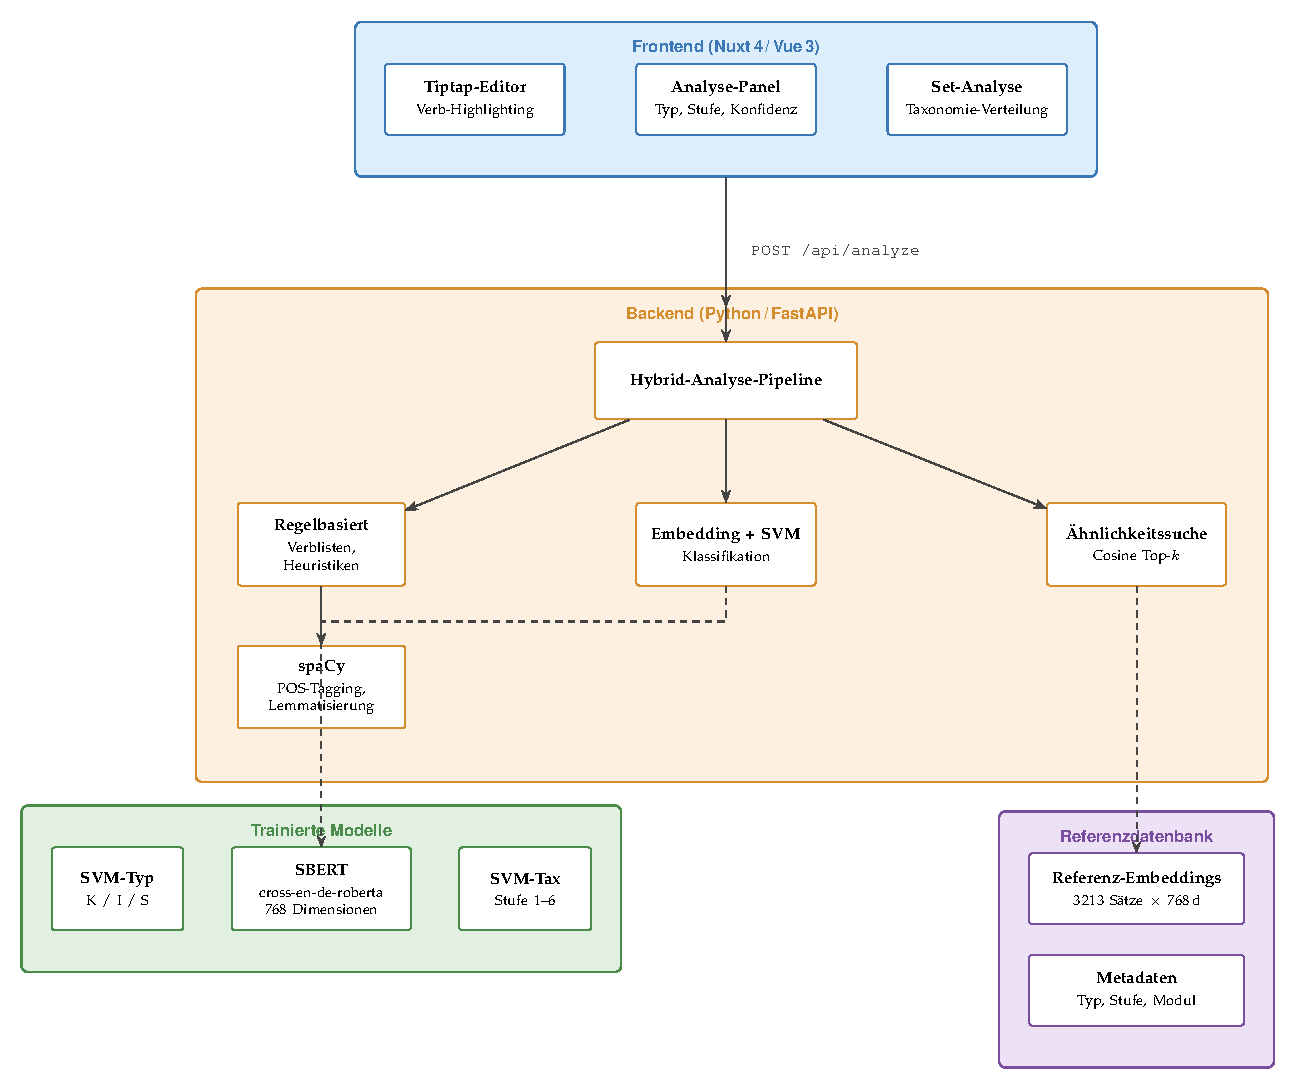
\includegraphics[width=\textwidth]{figures/architektur_gesamt.pdf}
\end{figure}

Die Schnittstelle zwischen Frontend und Backend ist bewusst minimal gehalten: Ein einzelner Endpunkt nimmt den Text entgegen und liefert alle Analyseergebnisse -- Satztyp, Taxonomiestufe, Konfidenz, erkannte Verben, ähnliche Formulierungen und Set-Analyse -- in einer JSON-Antwort zurück.
Diese Bündelung vermeidet mehrfache Roundtrips und vereinfacht die Frontend-Logik, da keine Zustandssynchronisation zwischen verschiedenen API-Aufrufen erforderlich ist.

Ergänzend stellt ein Health-Endpunkt (\texttt{GET /api/health}) den Ladestatus der Modelle bereit, sodass das Frontend den Systemzustand anzeigen kann.

\subsection{Hybrid-Cascading-Entwurf}\label{sec:cascading-entwurf}

Der Kern des Systems ist eine hybride Pipeline, die regelbasierte und Embedding-basierte Analyse in einem Cascading-Muster kombiniert.
Die Leitidee ist, für eindeutige Fälle die transparente und schnelle regelbasierte Zuordnung zu nutzen und nur für mehrdeutige oder unbekannte Fälle auf die kontextsensitive Embedding-Klassifikation zurückzugreifen.
Abb.~\ref{fig:cascading} zeigt den Ablauf.

\begin{figure}[t!]
\caption{Hybrid-Cascading-Pipeline. Regelbasierte Zuordnung greift bei eindeutigen Verben; bei mehrdeutigen oder unbekannten Verben wird die Embedding-basierte Klassifikation als Fallback eingesetzt.\label{fig:cascading}}
\centering
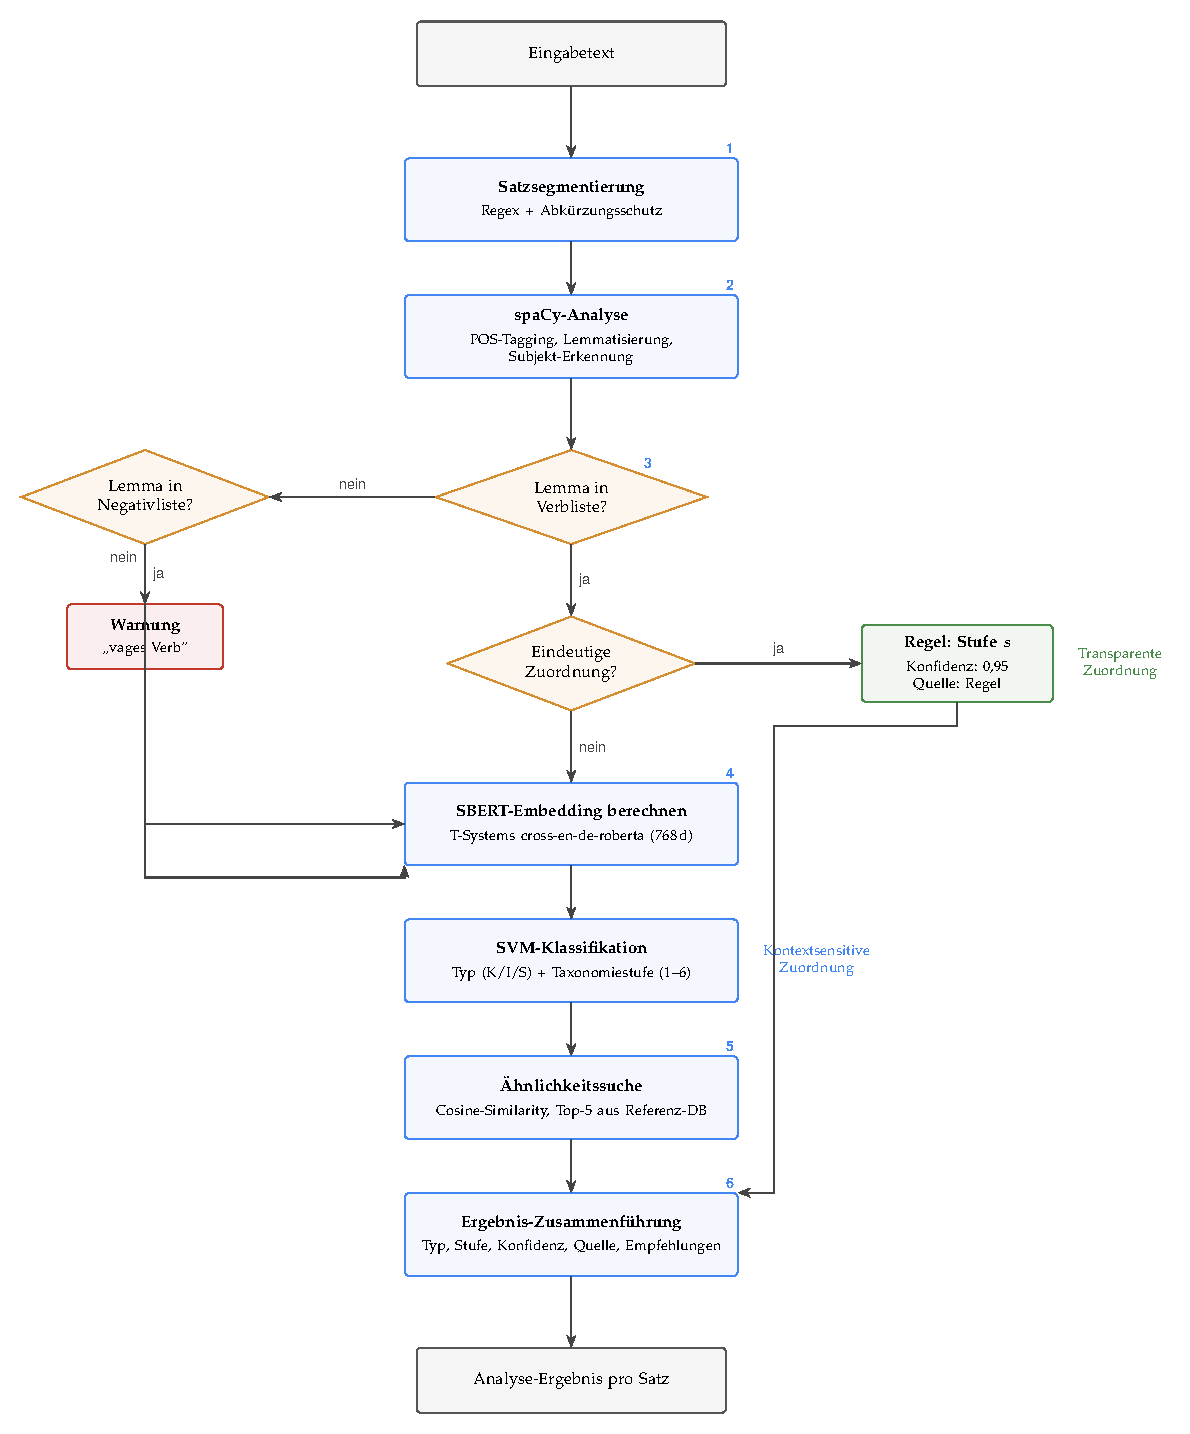
\includegraphics[width=0.72\textwidth]{figures/architektur_cascading.pdf}
\end{figure}

\subsubsection{Schritt 1: Satzsegmentierung}\label{sec:segmentierung}

Der Eingabetext wird in einzelne Sätze aufgeteilt.
Die Segmentierung verwendet spaCy, ergänzt um Schutzmechanismen für Abkürzungen (z.\,B., bzw., Prof., Dr.), die andernfalls zu falschen Satzgrenzen führen würden.
Aufzählungen und Infinitivkonstruktionen mit Semikolon werden als zusammengehörig behandelt.

\subsubsection{Schritt 2: Linguistische Vorverarbeitung}\label{sec:spacy-analyse}

Jeder Satz wird mit dem spaCy-Modell \texttt{de\_core\_news\_lg} analysiert.
Die Verarbeitung umfasst drei Aspekte: POS-Tagging zur Identifikation von Verben, Lemmatisierung zur Reduktion auf die Grundform und Subjekt-Erkennung zur Prüfung, ob \emph{die Studierenden} als Subjekt auftreten -- ein Indikator für eine Kompetenzformulierung.

\subsubsection{Schritt 3: Regelbasierte Klassifikation}\label{sec:regelbasiert}

Die regelbasierte Klassifikation operiert auf den extrahierten Verb-Lemmata und prüft diese gegen drei Listen: eine Positivliste empfohlener Verben mit Taxonomie-Zuordnung, eine Negativliste nicht empfohlener Verben und eine Liste von Modalverben.

Die Entscheidungslogik folgt einem kaskadierenden Schema.
Zunächst wird der \emph{Satztyp} bestimmt: Enthält der Satz ein erkanntes Subjekt (\emph{Studierende}) und mindestens ein Verb, wird er als Kompetenzformulierung (K) eingestuft; enthält er weder ein solches Subjekt noch ein Handlungsverb, wird er als Inhaltsbeschreibung (I) oder sonstiger Satz (S) klassifiziert.

Für als K klassifizierte Sätze wird anschließend die \emph{Taxonomiestufe} bestimmt.
Befindet sich das Lemma des Hauptverbs in der Positivliste und ist dort genau einer Stufe zugeordnet, wird diese Stufe direkt übernommen -- mit einer Konfidenz von 0{,}95 und der Quellenangabe \emph{Regel}.
Dieser Fall bildet den \emph{Short Circuit} des Cascading-Musters: Die Zuordnung ist abgeschlossen, ohne dass Embeddings berechnet werden müssen.

Ist das Verb zwar gelistet, aber mehreren Stufen zugeordnet (z.\,B. \emph{erkennen} auf Stufe~1, 2 und~4), oder befindet es sich nicht in der Positivliste, wird die Analyse an Schritt~4 delegiert.
Befindet sich das Verb in der Negativliste, wird zusätzlich eine Warnung erzeugt, die den Nutzenden auf die Verwendung eines unspezifischen Verbs hinweist.

\subsubsection{Schritt 4: Embedding-basierte Klassifikation}\label{sec:embedding-klassifikation}

Für alle Sätze, bei denen die regelbasierte Stufe keine eindeutige Zuordnung liefert, wird der vollständige Satz durch das SBERT-Modell in einen 768-dimensionalen Vektor überführt.
Auf diesem Embedding operieren zwei SVM-Klassifikatoren:

Der \emph{Typ-Klassifikator} ordnet den Satz den Klassen K, I oder S zu.
Er greift nur, wenn Schritt~3 keine eindeutige Typ-Bestimmung ergeben hat -- etwa bei Sätzen ohne erkanntes Subjekt, die dennoch Kompetenzformulierungen sein können (z.\,B. Passivkonstruktionen).

Der \emph{Taxonomie-Klassifikator} ordnet Kompetenzformulierungen einer der sechs Stufen nach Anderson und Krathwohl zu.
Er berücksichtigt den gesamten Satzkontext, nicht nur das isolierte Verb.
Dadurch kann er auch Verben korrekt einordnen, die je nach Kontext unterschiedlichen Stufen angehören -- eine Fähigkeit, die der regelbasierten Analyse prinzipbedingt fehlt.

Beide Klassifikatoren geben neben der Vorhersage eine Konfidenz aus, die aus der Wahrscheinlichkeitsschätzung der SVM (\texttt{predict\_proba}) abgeleitet wird.
Die Quellenangabe wechselt auf \emph{Embedding}.

\subsubsection{Schritt 5: Ähnlichkeitssuche}\label{sec:aehnlichkeitssuche}

Unabhängig von der Cascading-Entscheidung wird für jeden als Kompetenzformulierung klassifizierten Satz eine Ähnlichkeitssuche durchgeführt.
Das in Schritt~4 berechnete Embedding -- oder, falls der Satz bereits in Schritt~3 abgeschlossen wurde, ein nachträglich berechnetes Embedding -- wird gegen die Referenzdatenbank verglichen (vgl. Kap.~\ref{sec:referenz-db}).

Die Suche berechnet die Cosine-Similarity zwischen dem Eingabe-Embedding und allen Referenz-Embeddings und gibt die fünf ähnlichsten Formulierungen zurück, sortiert nach Similarity.
Für jede Empfehlung werden der Satztext, die Taxonomiestufe, der Similarity-Wert und die Herkunft (Modulname, Studiengang) angegeben.

\subsubsection{Schritt 6: Ergebnis-Zusammenführung}\label{sec:zusammenfuehrung}

Im letzten Schritt werden die Einzelergebnisse zu einem strukturierten Analyseergebnis pro Satz zusammengeführt.
Dieses enthält den Satztyp (K/I/S), die Taxonomiestufe (1--6 oder null), die Konfidenz (0--1), die Quelle (Regel oder Embedding), die erkannten Verben mit ihren Kategorien und Hervorhebungsklassen, die fünf ähnlichsten Referenzformulierungen sowie etwaige Warnungen.

Zusätzlich wird auf Textebene eine \emph{Set-Analyse} berechnet: Die Taxonomiestufen aller Kompetenzformulierungen werden aggregiert, die Abdeckung (Anzahl belegter Stufen) ermittelt und eine textuelle Empfehlung für fehlende Stufen generiert.
Diese Aggregation adressiert die Anforderung FA4 (Set-Analyse auf Modulebene).

\subsubsection{Cascading-Effizienz}\label{sec:cascading-effizienz}

Vom Cascading-Muster werden zwei Vorteile erwartet, die in Kap.~\ref{sec:kosten-nutzen} empirisch überprüft werden.
Erstens \emph{Transparenz}: Für Verben, die eindeutig in der Positivliste stehen, ist die Zuordnung direkt nachvollziehbar -- sie basiert auf einer expliziten Listenregel, nicht auf einer Blackbox-Klassifikation.
Die Quellenangabe (Regel vs. Embedding) macht für jeden Satz transparent, welches Verfahren die Zuordnung vorgenommen hat (NFA2).

Zweitens \emph{Performance}: Die regelbasierte Prüfung ist ein Dictionary-Lookup und benötigt unter 1\,ms.
Nur wenn dieser Lookup keine eindeutige Zuordnung liefert, wird die rechenintensivere Embedding-Berechnung ausgelöst.
Die Erwartung ist, dass Modulhandbücher überwiegend Standardverben enthalten und ein Großteil der Sätze den Short Circuit nutzen kann.
Tab.~\ref{tab:performance} zeigt die gemessenen Verarbeitungszeiten.

\begin{table}[H]
\caption{Verarbeitungszeiten der Pipeline-Schritte auf CPU\label{tab:performance}}
\centering
\small
\begin{tabular}{lrl}
\hline
\textbf{Schritt} & \textbf{Zeit} & \textbf{Anmerkung} \\
\hline
Satzsegmentierung & $<$\,1\,ms & Regex \\
spaCy POS-Tagging & $\sim$\,5\,ms/Satz & de\_core\_news\_lg \\
Regelbasierter Check & $<$\,1\,ms & Dictionary-Lookup \\
SBERT Encoding & $\sim$\,2\,ms/Satz & 546 Sätze/s (CPU) \\
SVM-Klassifikation & $<$\,1\,ms & Trainierte sklearn-Pipeline \\
Cosine-Similarity & $\sim$\,1\,ms & NumPy-Dot-Produkt \\
\hline
\textbf{Gesamt pro Satz} & $\sim$\,\textbf{10\,ms} & \\
\textbf{Typischer Modultext (5--10 Sätze)} & $\sim$\,\textbf{50--100\,ms} & Unter NFA5 ($<$\,2\,s) \\
\hline
\end{tabular}
\end{table}

\subsection{Modellauswahl}\label{sec:modellauswahl}

Die Wahl des Sentence-Embedding-Modells bestimmt maßgeblich die Klassifikationsleistung des Embedding-basierten Pfads.
Drei Kandidaten wurden systematisch evaluiert, die unterschiedliche Kompromisse zwischen Dimensionalität, Geschwindigkeit und Genauigkeit repräsentieren.

\subsubsection{Evaluierte Modelle}\label{sec:eval-modelle}

Alle drei Modelle sind vortrainierte Sentence-Transformer, die über die Hugging-Face-Plattform verfügbar sind und deutsche Texte unterstützen:

\begin{itemize}
  \item \textbf{paraphrase-multilingual-MiniLM-L12-v2} (384\,d): Ein kompaktes multilinguales Modell mit hoher Inferenzgeschwindigkeit (1\,859 Sätze/s), das durch Knowledge Distillation aus einem größeren Modell gewonnen wurde~\cite{reimers2020multilingual}.
  \item \textbf{deutsche-telekom/gbert-large-paraphrase-cosine} (1\,024\,d): Ein auf deutschem Text vortrainiertes BERT-Large-Modell mit der höchsten Dimensionalität, aber geringster Geschwindigkeit (203 Sätze/s).
  \item \textbf{T-Systems-onsite/cross-en-de-roberta-sentence-transformer} (768\,d): Ein cross-linguales RoBERTa-Modell, das auf englisch-deutschen Paraphrasen-Daten feinabgestimmt wurde und von der Reichhaltigkeit englischer Trainingskorpora profitiert.
\end{itemize}

\subsubsection{Evaluationsmethodik}\label{sec:eval-methodik-modelle}

Die Modellauswahl erfolgte auf dem initialen Datensatz der Hochschule Fulda (3\,213 Sätze, 80/20-Split, Seed~42), der zum Zeitpunkt der Entwurfsentscheidung vorlag.
Die finale Evaluation auf dem erweiterten, multiuniversitären Datensatz folgt in Kap.~\ref{sec:evaluation}.
Für jedes Modell wurde derselbe Klassifikator trainiert: eine SVM mit RBF-Kernel (C\,=\,10, gamma\,=\,scale) nach Standardisierung der Features (StandardScaler).
Die Hyperparameter wurden nicht optimiert, um einen fairen Vergleich der Embedding-Qualität -- unabhängig von Klassifikator-Tuning -- zu ermöglichen.
Als Metrik dient der gewichtete F1-Score auf dem Test-Split (641 Sätze).

\subsubsection{Ergebnisse und Entscheidung}\label{sec:modell-entscheidung}

Tab.~\ref{tab:modellvergleich} zeigt die Ergebnisse.

\begin{table}[H]
\caption{Vergleich der evaluierten Sentence-Embedding-Modelle\label{tab:modellvergleich}}
\centering
\small
\begin{tabular}{lrrrr}
\hline
\textbf{Modell} & \textbf{Dim} & \textbf{Sätze/s} & \textbf{Typ-F1} & \textbf{Tax-F1} \\
\hline
MiniLM-L12-v2 & 384 & 1\,859 & 0{,}977 & 0{,}846 \\
gbert-large & 1\,024 & 203 & 0{,}979 & 0{,}875 \\
\textbf{cross-en-de-roberta} & \textbf{768} & \textbf{546} & \textbf{0{,}977} & \textbf{0{,}906} \\
\hline
\end{tabular}
\end{table}

Alle drei Modelle erzielen bei der Typ-Klassifikation (K/I/S) nahezu identische Ergebnisse (F1 $\geq$ 0{,}977), was darauf hindeutet, dass die Unterscheidung zwischen Kompetenzformulierungen und Inhaltsbeschreibungen eine vergleichsweise einfache Aufgabe darstellt.
Die entscheidende Differenzierung zeigt sich bei der Taxonomie-Klassifikation: Hier übertrifft das cross-en-de-roberta-Modell von T-Systems das gbert-large-Modell um 3{,}1 Prozentpunkte und das MiniLM-Modell um 6{,}0 Prozentpunkte.

Das \textbf{T-Systems-onsite/cross-en-de-roberta-sentence-transformer} wird gewählt.
Die Entscheidung basiert auf drei Faktoren: (1)~die beste Taxonomie-Klassifikation (F1\,=\,0{,}906), die für die Kernfunktionalität des Systems ausschlaggebend ist; (2)~ein guter Kompromiss bei der Geschwindigkeit (546 Sätze/s -- 2{,}7$\times$ schneller als gbert-large); (3)~eine mittlere Dimensionalität (768\,d), die einen Kompromiss zwischen semantischer Ausdruckskraft und Speicherbedarf für die Ähnlichkeitssuche darstellt.

\subsubsection{SVM-Klassifikator-Architektur}\label{sec:svm-architektur}

Für beide Klassifikationsaufgaben wird eine sklearn-Pipeline aus StandardScaler und SVC mit RBF-Kernel eingesetzt.
Die Wahl der SVM folgt Kumar et al.~\cite{kumar2025automated}, die auf einem vergleichbaren Datensatz (Bloom-Taxonomie-Klassifikation englischer Lernergebnisse) zeigen, dass eine SVM auf Embeddings (94\,\% Accuracy) alle evaluierten Deep-Learning-Modelle übertrifft.
Die RBF-SVM ermöglicht durch die Kernelfunktion eine nichtlineare Entscheidungsgrenze im Embedding-Raum und gibt über die Platt-Skalierung (\texttt{probability=True}) kalibrierte Konfidenzwerte aus, die als Grundlage für die Konfidenzanzeige im Frontend dienen (NFA1).

Auf dem initialen Fulda-Datensatz (641~Test-Sätze) erreicht der Typ-Klassifikator (K/I/S) einen gewichteten F1-Score von 0{,}977 und der Taxonomie-Klassifikator (Stufen 1--6, nur K-Sätze) einen gewichteten F1-Score von 0{,}906.
Diese Werte dienen als Entwurfsgrundlage; die detaillierte Auswertung auf dem erweiterten Datensatz erfolgt in Kap.~\ref{sec:evaluation}.

\subsection{Referenzdatenbank}\label{sec:referenz-db}

Die Referenzdatenbank dient als Grundlage für die ähnlichkeitsbasierte Empfehlungsfunktion (FA3).
Sie enthält vorberechnete Embeddings aller Sätze aus dem Gold-Standard-Datensatz und ermöglicht eine effiziente Suche nach semantisch ähnlichen Formulierungen.

\subsubsection{Aufbau}

Die Datenbank besteht aus zwei Komponenten: einer Matrix normalisierter 768-dimensionaler Embedding-Vektoren (\texttt{.npy}-Datei) und einer JSON-Metadatendatei, die pro Satz den Text, den Satztyp, die Taxonomiestufe, den Modulnamen und den Studiengang speichert.
Die Embeddings werden mit demselben SBERT-Modell berechnet, das auch zur Laufzeit für Eingabesätze verwendet wird, um eine konsistente Repräsentation zu gewährleisten.

Die Normalisierung der Embedding-Vektoren auf Einheitslänge ist eine bewusste Entwurfsentscheidung: Für normalisierte Vektoren reduziert sich die Cosine-Similarity auf ein Dot-Produkt, das mit NumPy als Matrix-Vektor-Multiplikation in unter 1\,ms berechenbar ist.
Damit kann die Suche über alle Referenzen zur Laufzeit durchgeführt werden, ohne dass ein Approximate-Nearest-Neighbor-Index erforderlich wäre.

\subsubsection{Datengrundlage}

Die Referenzdatenbank wird aus dem Gold-Standard-Datensatz (vgl. Kap.~\ref{sec:eval-goldstandard}) aufgebaut, der über 5\,600~Sätze aus Modulhandbüchern von vier Hochschulen und vier Fachbereichen umfasst.
Die Annotation (Satztyp, Taxonomiestufe und Formulierungsqualität) erfolgte LLM-gestützt und wurde manuell validiert (vgl. Kap.~\ref{sec:eval-vorannotation}).
Die Referenzdatenbank nutzt den gesamten Datensatz -- nicht nur den Trainings-Split --, da bei der Ähnlichkeitssuche kein Klassifikator trainiert wird und somit kein Overfitting-Risiko besteht.
Durch die Einbeziehung externer Hochschulen deckt die Referenzdatenbank ein breiteres Spektrum an Formulierungsstilen ab und ermöglicht domänenübergreifende Empfehlungen.
